The \texttt{\pkglnk{view.exercise}} package contains the Application's exercise system:

The \texttt{\lnk{Exercise}} interface specifies that Exercises consist of a name, a task, a solution and (optional) predefined variables.
The \texttt{\lnk{ConcreteExercise}} class gives an implementation allowing for a simple generation of Exercises.
Note that Exercises use String representations of $\lambda$-Terms which must be transformed to \texttt{\hyperref[type:edu.kit.wavelength.client.model.term.LambdaTerm]{LambdaTerm}} objects when used.

The \texttt{\lnk{Exercises}} class static has only one method which statically returns a list of all available Exercises.

\begin{figure}[H]
	\centering
	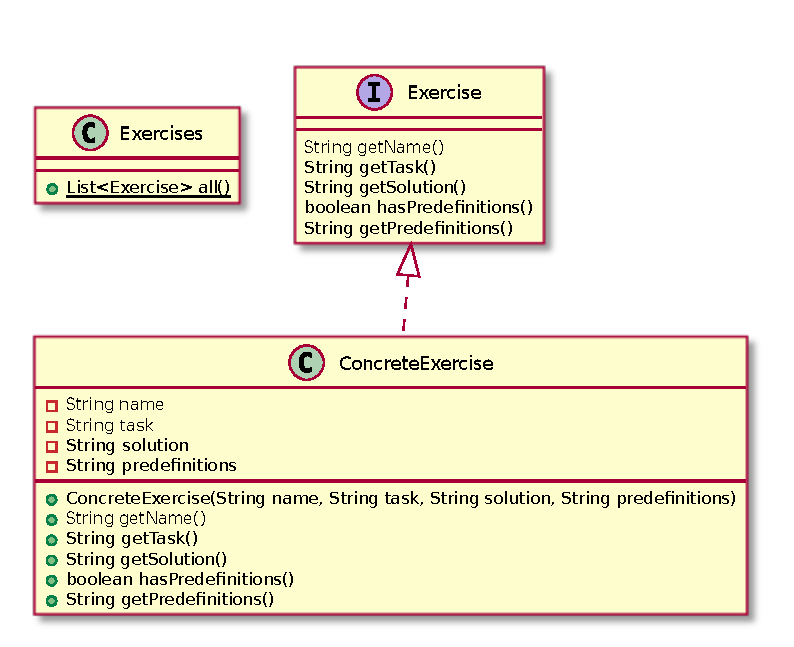
\includegraphics[width=\textwidth]{packageDiagrams/exercisePackage}
\end{figure}

